\documentclass[11pt,a4paper]{article}
\usepackage[utf8]{inputenc}
\usepackage{amsmath, mathtools}
\usepackage{amsfonts, dsfont}
\usepackage{amssymb}
\usepackage{graphicx}
\usepackage{empheq}
\usepackage{bm}
\usepackage[round, sort]{natbib}
\usepackage{tikz}
\usepackage{mathtools}  
\mathtoolsset{showonlyrefs}  
\usetikzlibrary{shapes,backgrounds,arrows,automata,snakes,shadows,positioning, mindmap}

%%%%% Commands
\newcommand{\argmin}{\arg\!\min}
\newcommand{\argmax}{\arg\!\max}
\newcommand*\widefbox[1]{\fbox{\hspace{3em}#1\hspace{3em}}}
\newcommand*\lesswidefbox[1]{\fbox{\hspace{2em}#1\hspace{2em}}}
\newcommand{\entr}{\mathcal{H}}
\newcommand{\betabf}{\boldsymbol{\beta}}
\newcommand{\thetabf}{\boldsymbol{\theta}}
\newcommand{\mubf}{\boldsymbol{\mu}}
\newcommand{\Omegabf}{\boldsymbol{\Omega}}
\newcommand{\Sigmabf}{\boldsymbol{\Sigma}}
\newcommand{\zerobf}{\boldsymbol{0}}
\newcommand{\Xbf}{\boldsymbol{X}}
\newcommand{\xbf}{\boldsymbol{x}}
\newcommand{\Ybf}{\boldsymbol{Y}}
\newcommand{\Zbf}{\boldsymbol{Z}}
\newcommand{\Sbf}{\boldsymbol{S}}
\newcommand{\mbf}{\boldsymbol{m}}
\newcommand\Ncal{\mathcal{N}}
\newcommand\Pcal{\mathcal{P}}
\newcommand\Tcal{\mathcal{T}} 
\newcommand{\Esp}{\mathds{E}}
\newcommand{\bound}{\mathcal{J}}
 
 %%%%%%% TIKZ
 \newcommand{\edgeunit}{1.5}
\providecommand\given{} % is redefined in \Set
\newcommand\SetSymbol[1][]{\nonscript\:#1\vert\nonscript\:}
%\usepackage[mathcal]{eucal}
\usepackage[left=2cm,right=2cm,top=2cm,bottom=2cm]{geometry}
\tikzset{%
    observed/.style={%
    scale=0.9,rectangle,draw=white,transform shape,fill=white,font=\Large}
}
\tikzset{%
    basic/.style={%
    scale=0.9,circle,draw=black,transform shape,fill=white,font=\small}
}


\setlength\parindent{0pt}
\author{Raphaelle Momal}
\title{PLN with missing actor}

 

\begin{document}

\maketitle
\vspace{3cm}
\tableofcontents
\newpage
Previously:
$$ p(Y,Z,T) = p(T)p(Z|T)p(\Ybf|Z)$$
$$ \Esp(\log p(\Ybf,Z,T)|\Ybf) \approx \sum_{1 \leq j < k \leq p} P_{jk} \log\left(\beta_{jk} \hat{\psi}_{jk}\right) - \log B + cst$$

Now adding a hidden layer of unobserved data, indexed by H:

$$ p(\Ybf,Z_O,Z_H,T)$$
\section{PLNmissing peculiarities:}

\subsection{Model}

$$\left\{\begin{array}{rl}
T & \sim\prod_{jk \in T} \beta_{jk}/B \\\\
Z|T& \sim\mathcal{N}(0,\Sigma_T)\\\\
\Ybf|Z&\sim\mathcal{P}( \exp( Z+...) )
\end{array} \right.$$

\paragraph{Dimensions:}
The model is build on matrices $\Ybf$ and $Z$ with the following dimensions:\\
$\Ybf$: $n\times p$\\
$Z_O$: $n\times p$\\
$Z_H$: $n\times r$


\paragraph{Underlying dependencies:} This diagram is the graphical model behind the model, it describes the variables direct denpendencies and how data is simulated. Here, a tree $T$ is first drawn, which controls the dependency structure of parameters $Z = (Z_O,Z_H)$. Count data $\Ybf$ is drawn from a distribution depending only on observed parameters $Z_O$.
\begin{center}
	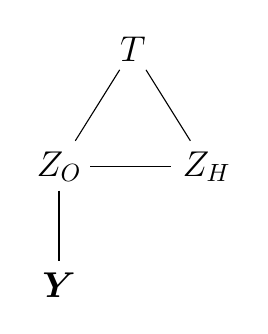
\begin{tikzpicture}	
      \tikzstyle{every edge}=[-,>=stealth',shorten >=1pt,auto,thin,draw]
		\node[observed] (A1) at (0.625*\edgeunit, 2*\edgeunit) {$T$};
		\node[observed] (A2) at (0*\edgeunit, 1*\edgeunit) {$Z_O$};
		\node[observed] (A3) at (1.25*\edgeunit, 1*\edgeunit) {$Z_H$};
		\node[observed] (A4) at (0*\edgeunit, 0*\edgeunit) {$\Ybf$};
		\path (A1) edge [] (A2)
        (A1) edge [] (A3)
        (A2) edge [] (A3)
        (A2) edge [] (A4);
	\end{tikzpicture}
\end{center}

\subsection{Distributions}
\paragraph{Marginals}
The complete vector of underlying parameters $Z$ follows a mixture of Gaussian laws on the space of all existing spanning trees.
\begin{align*}
(Z_O,Z_H) &\sim \sum_{T \in \mathcal{T}} p(T) \mathcal{N}(0,\Sigma_T) \\
\end{align*}

\paragraph{Conditional on T:}
Conditionally on the dependency structure $T$, $Z$ is a centered Gaussian variable, with covariance matrix $\Sigma_T$ defined by block:
\[
 \Sigma=
  \left( {\begin{array}{cc}
  \Sigma_{TO} &  \Sigma_{TOH}\\\\
  \Sigma_{THO} & \Sigma_{TH}
  \end{array} } \right) =
   \left( {\begin{array}{cc}
  \Omega_{TO} &  \Omega_{TOH}\\\\
  \Omega_{THO} & \Omega_{TH}
  \end{array} } \right)^{-1}
  \]\\
This results in the following distributions:
\begin{align*}
(Z_O,Z_H)|T & \sim\mathcal{N}(0,\Sigma_T)\\
Z_O|T & \sim\mathcal{N}(0,\Omega_{Tm}^{-1})\\
Z_H|T & \sim\mathcal{N}(0,\Omega_{Tm_H}^{-1})
\end{align*}
With $ \Omega_{Tm} =\Sigma_{TO}^{-1} =  \Omega_{TO} - \Omega_{TOH}\Omega_{TH}^{-1}\Omega_{THO}$, and $\Omega_{Tm_H} = \Sigma_{TH}^{-1} = \Omega_{TH} - \Omega_{THO} \Omega_{TO}^{-1} \Omega_{TOH}$. This comes from the Schur's complement which is recalled here:


\begin{align*}
 \Sigma_T=
  \left( {\begin{array}{cc}
  \Omega_{TO} &  \Omega_{TOH}\\\\
  \Omega_{THO} & \Omega_{TH}
  \end{array} } \right)^{-1} &=
  \left( {\begin{array}{cc}
  \Sigma_{TO} =( \Omega_{TO} - \Omega_{THO}\Omega_{TH}^{-1}\Omega_{TOH})^{-1} &  - \Sigma_{TO} \Omega_{TOH}\Omega_{TH}^{-1}\\\\
 -\Omega_{TH}^{-1}\Omega_{THO}\Sigma_{TO} & \Omega_{TH}^{-1}+\Omega_{TH}^{-1}\Omega_{TOH}\Sigma_{TO}\Omega_{THO}\Omega_{TH}^{-1}
  \end{array} } \right)\\\\
  &=   \left( {\begin{array}{cc}
   \Omega_{TO}^{-1}+\Omega_{TO}^{-1}\Omega_{TOH}\Sigma_{TH}\Omega_{THO}\Omega_{TO}^{-1} & -\Omega_{TO}^{-1}\Omega_{TOH}\Sigma_{TH} \\\\
    -\Sigma_{TH}\Omega_{THO}\Omega_{TO}^{-1}&  \Sigma_{TH}= (\Omega_{TH} - \Omega_{THO}\Omega_{TO}^{-1}\Omega_{TOH})^{-1} 
   \end{array} } \right)
\end{align*}
  


\paragraph{Conditional on observed data:\\}


As $Z_O$ decouples $Z_H$ and $\Ybf$, we will never need $Z_H|\Ybf$:
$$ p(Z|\Ybf) = p(Z_O,Z_H | \Ybf) = p(Z_H|Z_O) \: p(Z_O|\Ybf) $$



Model for the hidden part: $$Z_H|Z_O,T \sim \mathcal{N}(\mu_{H|O,T}, \Omega_{H}^{-1})$$ 

\begin{itemize}
\item In a precision matrix of a multivariate Gaussian, the conditional bloc is the marginal bloc:  $\Omega_{TH|O}^{-1} = \Sigma_{TH} -\Sigma_{THO}\Sigma_{TO}^{-1}\Sigma_{TOH} = \Omega_{TH}^{-1}$. Moreover the H block of $\Omega_T$ is diagonal as imposed by identifiability conditions (two hidden nodes cannot be linked with each other), and diagonal terms are assumed to not depend on tree $T$. Hence $\Omega_{TH|O}^{-1}=\Omega_{H}^{-1}$.

\item let's $Z_{Oi}$ denote a realization of $\mathcal{N}(0,\Sigma_{TO}) $.\\
 Then $\displaystyle  \mu_{H|Oi,T} = \Sigma_{THO}\Sigma_{TO}^{-1}(Z_{Oi}-\underbrace{\mu_{Z_Oi|T}}_{0}) 
 = -\Omega_{TH}^{-1}\Omega_{THO} \: Z_{Oi}
$\\
\end{itemize}



\section{Variational EM inference}
\subsection{Approximation of the likelihood}
\paragraph{Joint likelihood:}
The graphical model gives the following writing of the joint likelihood:
\begin{align*}
p(\Ybf,Z,T)& = p(T) \: p(Z|T) \: p(\Ybf|Z) \\
&= p(T)\: p(Z_O,Z_H|T) \: p(\Ybf|Z_O,Z_H) \\
&= p(T) \: p(Z_O|T) \: p(Z_H | Z_O,T)  \: p(\Ybf|Z_O)
\end{align*} 


\paragraph{Variational approximation:}

Here $p(T,\Zbf \mid \Ybf)$ is untractable. We adopt a variational approximation aiming to maximise a lower bound of the log-likelihood of observed data $\log p(\Ybf)$, namely  
\begin{align*}
    \mathcal{J}(\Ybf; g,h)
    & = \log p(\Ybf) - KL\left[q(T,\Zbf) \middle\vert\middle\vert\ p(T,\Zbf \mid \Ybf)\right]\\
    & =\Esp_{q}\big[\log p_{\thetabf}(\Ybf\mid \Zbf_O)+ \log p_{\Omegabf_T}(\Zbf_O \mid T)\big]-\Esp_q[\log h(\Zbf_O)]  +\Esp_{q}[\log p_{\Omegabf_T}(\Zbf_H \mid \Zbf_O,T)] \\
    & \;\; +\Esp_q\big[\log p_{\betabf}(T) - \log g(T)\big]  -\Esp_q[\log h(\Zbf_H)]
\end{align*}
Where KL is the Küllback-Leibler divergence. The approximation we adopt relies on factorizing $q$ in the product of two distributions $h$ et $g$ relating respectively to $\Zbf$  and $T$: 
$$p(T,Z | \Ybf) \approx  q(Z,T) = g(T)h(Z).$$

 A consequence of this hypothesis is the contributions of   $\Esp_h[\log p(\Zbf\mid T)]$ ainsi que $\log p(T)$ --~seuls termes qui font intervenir $T$ dans la borne inférieure~-- writing as sums on the edges. As distribution   $g$ minimizes the KL divergence, it has to factorizes on the edges as well. Hence:
$ g(T) = \left(\prod_{kl} \widetilde{\beta}_{kl} \right) / \widetilde{B}$. \\
 
Moreover, De plus, it follows from the independence of the samples that $h$ is a product law: $ h(\Zbf) = \prod_i h_i(\Zbf_i)$.
Our variational approximation consists in assuming that each of its components is a multivariate Gaussian: $h(\Zbf_i) = \Ncal(\Zbf_i; \mbf_i, \Sbf_i)$, where $\Sbf_i$ is diagonal. More precisely:  $ h(Z_i) =  \mathcal{N}(m_i,S_i)$ , where $S_i$ is diagonal with diagonal $(s_{i1}^2, ... , s_{i(p+r)}^2)$, meaning that $Z_H$ and $Z_O$ are independant. Marginals are written $h_O$  and  $h_H$. $S=\sum_i S_i$  and $ M =  [m_i]_{1 \leq i \leq (p+r)}$ (so $\Esp_h[Z_{\cdot k}^\intercal Z_{\cdot k}] = \sum_i s_{ik} + m_{\cdot k}^\intercal m_{\cdot k}$). $S$ is also diagonal and its H and O blocs are denoted $S_H$ and $S_O$. 

In the following we use the scalar product on the matrix space defined with the trace operator as: 
$$  Tr(A^\intercal B) = <A,B> .$$
\paragraph{Lower bound:}
Starting with the two hidden layers of our model, the lower bound writes:
\begin{align*}
\mathcal{J}(\Ybf; g,h)&=\log p(\Ybf) - KL\left[g(T) h(\Zbf) \middle\vert\middle\vert\ p(T,\Zbf | \Ybf)\right]\\
&= \log p(\Ybf) - \Esp_{gh}[\log( g(T) h(\Zbf)) - \log p(\Zbf,T\mid \Ybf) ]\\
&= \log p(\Ybf) - \Esp_{gh}[\log g(T) + \log h(\Zbf) ] + \Esp_{gh}[\log p(\Ybf,\Zbf,T)] - \Esp_{gh}[\log p(\Ybf)]\\
&= \Esp_{gh} [\log p(\Ybf,\Zbf,T)] + \entr[g(T)] + \entr[h(\Zbf)]\\
&= \Esp_{gh} [\log (p_\beta(T)p_{\Omega_T}(\Zbf\mid T)p_\theta(\Ybf\mid \Zbf))] + \entr[g(T)] + \entr[h(\Zbf)]
\end{align*}

Adding modelization of unobserved covariates:
\begin{align*}
\mathcal{J}(\Ybf; g,h)&= \Esp_{gh}[\log p(T)  p(\Zbf_H| \Zbf_O,T) p(\Zbf_O|T)p(\Ybf|\Zbf_O)] + \entr[g(T)] +\entr[h(\Zbf_H,\Zbf_O)]
\end{align*}

 We develop the entropy of the complete $\Zbf$ vector, to make the entropy of the fully observed part appear:
\begin{align*}
\entr[h(\Zbf_H,\Zbf_O)] &= -\Esp_h[\log h(\Zbf_H,\Zbf_O)]\\
&=-\Esp_h[\log h(\Zbf_H\mid \Zbf_O) h(\Zbf_O)]\\
&=\entr[h(\Zbf_O)] -\Esp_h[\log h(\Zbf_H\mid \Zbf_O)]
\end{align*}

Now using the hypothesis of independence of $g$ and $h$, we can obtain quantities with seperate dependencies:

\begin{align*}
\mathcal{J}(\Ybf; g,h)&=   \Esp_{gh}[\log p(\Zbf_H | \Zbf_O,T)  p(\Zbf_O | T)] +\Esp_g[\log p(T)] + \Esp_h[\log p(\Ybf|\Zbf_O)]-\Esp_h[\log h(\Zbf_H\mid \Zbf_O)]&\\
& \;\; + \entr[g(T)] +\entr[h(\Zbf_O)] 
\end{align*}




%Property of Shannon entropy : $\entr(X,\Ybf) = \entr(X) + \entr(\Ybf|X)$

Finally we obtain:

\begin{align}
\mathcal{J}(\Ybf; g,h)&=  \Esp_{gh}[\log p(\Zbf_O | T)] +\Esp_h[\log p(\Ybf|\Zbf_O)]+\entr[h(\Zbf_O)]& \text{: PLN like} \nonumber\\
& \;\; + \Esp_{gh}[\log p(\Zbf_H | \Zbf_O,T) ]+\Esp_g[\log p(T)] +\entr[g(T)]-\Esp_h[\log h(\Zbf_H\mid \Zbf_O)]&\text{: New}\label{lowerbound}
\end{align}\\

\subsection{Optimizing in $\theta$ and $h(\Zbf_O)$:}
\citet{CMR18} compute the lower bound of a VEM for the PLN, which we write $\mathcal{J}_{PLN}$. This lower bound appears in our computation as well. Let's first detail the following quantity:
\begin{align*}
\Esp_{gh}[\log p(\Zbf_O|T)] &=  \Esp_{gh} \left[\frac{n}{2} \log |\Omega_{Tm}| - \frac{1}{2} \sum_i \Zbf_{Oi}\Omega_{Tm} \Zbf_{Oi}^\intercal  \right]\\
&= \frac{n}{2} \Esp_g [\log |\Omega_{Tm}|] - \frac{1}{2} \Esp_{gh}\left[Tr\left( \Zbf_O^\intercal \Zbf_O \Omega_{Tm}\right)\right].
\end{align*}

The expectation in $gh$ is separable thanks to the independance hypothesis:
\begin{align*}
\Esp_{gh}[\log p(\Zbf_O|T)] &=\frac{n}{2} \Esp_g [\log |\Omega_{Tm}|] - \frac{1}{2}  Tr\left(\Esp_h [\Zbf_O^\intercal \Zbf_O ]\; \Esp_g[\Omega_{Tm}]\right)\\
&=\frac{n}{2} \Esp_g [\log |\Omega_{Tm}|] - \frac{1}{2}<\Esp_h [\Zbf_OZ_O^\intercal ], \underbrace{\Esp_g [\Omega_{Tm}]}_{\overline{\Omega_{Tm}}}> .
\end{align*}
We note $\Esp_g [\Omega_{Tm}] = \overline{\Omega_{Tm}}$, which is a $p\times p$ matrix of expected covariance over the whole spanning-tree space. Introducing the quantity  $\log |\overline{\Omega_{Tm}}| $ in the PLN-like terms of Eq.~(\ref{lowerbound}), the lower bound of the VEM of PLN $\mathcal{J}_{PLN}$ appears:
\begin{align*}
&\Esp_{gh}[\log p(\Zbf_O | T)] +\Esp_h[\log p(\Ybf|\Zbf_O)]+ \entr[h(\Zbf_O)]\\
& =\underbrace{\frac{n}{2} \log |\overline{\Omega_{Tm}}| - \frac{1}{2}<\Esp_h [\Zbf_OZ_O^\intercal ], \overline{\Omega_{Tm}}> + \Esp_{h}[\log p(\Ybf|\Zbf_O)] + \entr[h(\Zbf_O)]}_{\mathcal{J}_{PLN}\text{ with } \widetilde{\Sigma} = \overline{\Omega_{Tm}}} + \underbrace{\frac{n}{2}\left( \Esp_g[\log|\Omega_{Tm}|] - \log|\overline{\Omega_{Tm}}|\right)}_{\leq 0}
\end{align*}


The second brace is a negative quantity, because the log determinent is a concave function. Jensen's inequality gives:
$$\log |\Esp_g[\Omega_{Tm}]| \geq \Esp_g [\log |\Omega_{Tm}|]$$
%$$ \Esp[Z_jZ_k] = -\partial_{\omega_{jk}}( \log |\Omega_{TO}| )$$
Therefore, $$\Esp_{gh}[\log p(\Zbf_O | T)] +\Esp_h[\log p(\Ybf|\Zbf_O)]+ \entr[h(\Zbf_O)] \leq \mathcal{J}_{PLN}$$\\
\begin{align*}
\mathcal{J}_{h}(\Ybf; g,h)&= \mathcal{J}_{PLN}+\frac{n}{2}\left(\Esp_g[\log|\Omega_{Tm}|] - \log|\overline{\Omega_{Tm}}|\right)\\
&\;+ \Esp_{gh}[\log p(\Zbf_H | \Zbf_O,T) ]+\Esp_g[\log p(T)] +\entr[g(T)]-\Esp_h[\log h(\Zbf_H\mid \Zbf_O)]
\end{align*}
The "VE" step of PLNmodels algorithm maximizes $\mathcal{J}_{PLN}$ and gives estimates of $\Zbf_O$ moments of order 1 and 2. So we have easy access to $\widetilde{m}_O, \widetilde{S}_O, \widetilde{\overline{\Omega_{Tm}}}$, which maximize part of $\mathcal{J}(\Ybf;g,h)$ in $h(\Zbf_O)$.  \\

Remarks:
\begin{itemize}
\item Here it shows that assuming a tree structure for the latent layer of parameters $\Zbf$ reveals an average precision matrix over all the precision matrices of possible trees. Recall that these matrices only differ in the position of their zero entries.
\item Not all terms depending on $h(\Zbf_O)$ are in $\mathcal{J}_{PLN}$, so the proposed solution is sub-optimal. After maximizing $\mathcal{J}_{PLN}$ in $h_O$, this density is considered constant and written $h_O^*$.  
\end{itemize}




\subsection{VE step: optimizing in $g$ and $h(\Zbf_H)$}
The VE step minimizes the Küllback-Leibler divergence between the approximated and the aimed distributions :

$$  \argmin_{g,h(\Zbf_H)} KL\left(g(T)h(\Zbf) || p(\Zbf,T|\Ybf)\right)$$


\begin{align*}
KL\left(g(T)h(\Zbf) || p(\Zbf,T|\Ybf)\right) &= \Esp_{gh}\left[\log g(T)h(\Zbf) - \log p(\Zbf,T\mid \Ybf) \right]\\
&= \Esp_{gh}\left[\log g(T)h(\Zbf) - \log p(\Ybf,\Zbf,T) + \log p(\Ybf)  \right]\\
&= \Esp_{gh}\left[\log g(T)+ \log h(\Zbf) - \log (p(T)p(\Zbf\mid T) p(\Ybf\mid \Zbf)) + \log p(\Ybf)  \right]\\
&=\Esp_{gh}\left[\log g(T) + \log h(\Zbf_O)+ \log h(\Zbf_H|\Zbf_O) - \log p(T)- \log p(\Zbf_H|\Zbf_O,T)\right. \\
& \;\;\;- \log p(\Zbf_O|T)- \log p(\Ybf|\Zbf_O)+ \log p(\Ybf) )\left. \right]
\end{align*}
The aim is to minimize with respect to distributions $g$ and $h(\Zbf_H)$. As distributions $p(\Ybf)$, $p(\Ybf\mid \Zbf_O)$ and $h(\Zbf_O)$ do not depend on them, we obtain:
\begin{align*}
\argmin_{g,h(\Zbf_H)} KL  &=\argmin_{g,h(\Zbf_H)} \Big\{ \Esp_{gh}\big[\log g(T) + \log h(\Zbf_H|\Zbf_O) - \log p(T)- \log p(\Zbf_H|\Zbf_O,T)-\log p(\Zbf_O|T) \big]\Big\}
\end{align*}
Under distribution $h$, $\Zbf_H$ and $\Zbf_O$ are independent, so $h(\Zbf_H\mid \Zbf_O) = h(\Zbf_H)$. Finally using the partly optimal distribution $h_O^*$ for $h(\Zbf_o)$, we obtain:

\begin{empheq}[box=\widefbox]{align*}
\argmin_{g,h(\Zbf_H)} KL  &=\argmin_{g,h(\Zbf_H)}  \Big\{- \Esp_{gh}[ p(\Zbf_H|\Zbf_O,T)] - \Esp_{gh_O^*}[\log p(\Zbf_O|T)] + \Esp_g\big[\log g(T)-\log p(T)\big]\\
& \hspace{2.5cm} + \Esp_h[\log h(\Zbf_H)]  \Big\}
\end{empheq}

\subsubsection{Details of  $-\Esp_{gh}[\log p(\Zbf_H | \Zbf_O,T) ]$}
Recalling $\mu_{H|Oi,T} = -\Omega_H^{-1}\Omega_{THO}\Zbf_{Oi} ^\intercal $ and that $\Omega_H$ is constrained to be diagonal and indenpendent of $T$ for identifiability, we have:
\begin{align*}
\log p(\Zbf_H\mid \Zbf_O,T) &= \frac{n}{2} \log |\Omega_H| -\frac{1}{2} \sum_i (\Zbf_{Hi}-\mu_{H|Oi,T}^\intercal )\Omega_H(\Zbf_{Hi}-\mu_{H|Oi,T}^\intercal )^\intercal \\
&= \frac{n}{2} \log |\Omega_H| -\frac{1}{2} \sum_i \left(\Zbf_{Hi}\Omega_HZ_{Hi}^\intercal  + \mu_{H|Oi,T}^\intercal \Omega_H\mu_{H|Oi,T} - 2\mu_{H|Oi,T}^\intercal \Omega_HZ_{Hi} \right)\\
&= \frac{n}{2} \log |\Omega_H| -\frac{1}{2} \sum_i \left(\Zbf_{Hi}\Omega_HZ_{Hi}^\intercal  + \Zbf_{Oi}\Omega_{TOH}\Omega_H^{-1} \Omega_{THO}\Zbf_{Oi}^\intercal + 2Z_{Oi}\Omega_{TOH}\Zbf_{Hi}^\intercal\right)\\
&=\frac{n}{2} \log |\Omega_H| -\frac{1}{2}Tr(\Zbf_H\Omega_HZ_H^\intercal) - \frac{1}{2}Tr(\Zbf_O\Omega_{TOH}\Omega_H^{-1}\Omega_{THO}\Zbf_o^\intercal) - Tr(\Zbf_O\Omega_{TOH}\Zbf_H^\intercal)
\end{align*}


Now taking the expectation, and by independence of $g$ and $h$:
\begin{align*}
\Esp_{gh}[\log p(\Zbf_H | \Zbf_O,T) ] &=\frac{n}{2} \log |\Omega_H| -\frac{1}{2}Tr(\Esp_{gh}[\Zbf_H\Omega_HZ_H^\intercal]) - \frac{1}{2}Tr(\Esp_{gh}[\Zbf_O\Omega_{TOH}\Omega_H^{-1}\Omega_{THO}\Zbf_O^\intercal]) \\
& \;\;\;- Tr(\Esp_{gh}[\Zbf_O\Omega_{TOH}\Zbf_H^\intercal])\\
&=\frac{n}{2} \log |\Omega_H| -\frac{1}{2} <\Omega_H,\Esp_h[\Zbf_H^\intercal \Zbf_H]> -\frac{1}{2} <\Esp_g[\Omega_{THO}^\intercal \Omega_H^{-1}\Omega_{THO}],\Esp_{h_O^*}[\Zbf_O^\intercal \Zbf_O]> \\
&\;\;\; -<\Esp_g[\Omega_{TOH}],\Esp_h[\Zbf_H^\intercal \Zbf_O]>
\end{align*}\\

Moreover we have :
\[\left\{\begin{array}{ll}
\Esp_h[\Zbf_H^\intercal \Zbf_H] &= M_H^\intercal M_H + S_H\\
\Esp_{h_O^*}[\Zbf_O^\intercal \Zbf_O] &= \widetilde{M}_O^\intercal \widetilde{M}_ O + \widetilde{S}_ O\\
\Esp_h[\Zbf_H^\intercal \Zbf_O] &= M_H^\intercal \widetilde{M}_O + \underbrace{S_{HO}}_{=0}
\end{array} \right.\]

Therfore, we obtain:

\begin{empheq}[box=\widefbox]{align*}
-\Esp_{gh}\big[\log p(\Zbf_H\mid \Zbf_O)\big] &= -\frac{n}{2} \log |\Omega_H| + \frac{1}{2}<\Omega_H, M_H^\intercal M_H + S_H> + \frac{1}{2}<\Esp_g\big[\Omega_{TOH}\Omega_H^{-1}\Omega_{THO}\big],\widetilde{M}_O^\intercal \widetilde{M}_ O + \widetilde{S}_ O> \\
& \;\;\;+ <\Esp_g[\Omega_{TOH}],M_H^\intercal \widetilde{M}_O>
\end{empheq}




\subsubsection{Detials of $-\Esp_{gh_O^*}[\log p(\Zbf_O|T)]$}
Recall that $Z_O|T sim \mathcal{N}(0,\Omega_{Tm}^{-1})$, where $\Omega_{Tm} = \Omega_{TO} - \Omega_{TOH}\Omega_H^{-1} \Omega_{THO} $. Hence:
\begin{align*}
\log p(Z_O|T) &= \frac{n}{2} \log |\Omega_{Tm}| - \frac{1}{2}Tr(\Omega_{Tm}\Zbf_O^\intercal \Zbf_O)\\
&=\frac{n}{2} \log |\Omega_{Tm}| - \frac{1}{2} Tr(\Omega_{TO}\Zbf_O^\intercal \Zbf_O) + \frac{1}{2} Tr((\Omega_{TOH}\Omega_H^{-1}\Omega_{THO}) \Zbf_O^\intercal \Zbf_O)
\end{align*}
Then, taking the expectation in $g$ and $h_O*$:
\begin{align*}
 \Esp_{gh_O^*}[\log p(\Zbf_O|T)] &= \frac{n}{2} \Esp_g[\log |\Omega_{Tm}|] - \frac{1}{2} < \Esp_g[\Omega_{TO}], \Esp_{h_O^*}[ \Zbf_O^TZ_O] >  + \frac{1}{2}<\Esp_g\big[\Omega_{TOH}\Omega_H^{-1}\Omega_{THO}\big],\Esp_{h_O^*}[ \Zbf_O^TZ_O]> 
\end{align*}
 
Because $\Omega_{Tm}$ is tree-structured, its determinent factorizes on the edges of $T$. More precisely as in \citet{robin2019}:
\begin{align*}
|\Omega_{Tm}| &= \prod_{k\in O} \omega_{kk} \prod_{kl \in T} \frac{\omega_{kk}\omega_{ll}-\omega_{kl}^2}{\omega_{kk}\omega_{ll}}\\
\log |\Omega_{Tm}|&= \sum_{k\in O} \log \omega_{kk} + \sum _{kl} \mathds{1}\{kl \in T\} \left[\log\frac{\omega_{kk}\omega_{ll}-\omega_{kl}^2}{\omega_{kk}\omega_{ll}}\right]\\
\Esp_g[\log |\Omega_{Tm}|]&= \sum _{kl} P_{gkl} \log \left[\frac{\omega_{kk}\omega_{ll}-\omega_{kl}^2}{\omega_{kk}\omega_{ll}}\right] + \sum_{k\in O} \log \omega_{kk}
\end{align*}

Finally we obtain:
\begin{empheq}[box=\widefbox]{align*}
- \Esp_{gh_O^*}[\log p(\Zbf_O|T)] &= -\frac{n}{2}\sum_{k\in O} \log \omega_{kk}+\sum _{kl} P_{gkl}  \log\left(1- \frac{ \omega_{kl}^2}{\omega_{kk}\omega_{ll}}\right)^{-\frac{n}{2}} + \frac{1}{2}<\Esp_g[\Omega_{TO}],\widetilde{M}_O^\intercal \widetilde{M}_O + \widetilde{S}_O>\\
&\;\;\; - \frac{1}{2}<\Esp_g\big[\Omega_{TOH}\Omega_H^{-1}\Omega_{THO}\big],\widetilde{M}_O^\intercal \widetilde{M}_O + \widetilde{S}_O>
\end{empheq}

\subsubsection{Details of $\Esp_g[\log g(T) - \log p(T)]$}
\begin{align*}
\log g(T) - \log p(T) &= \left(  \sum_{jk} \mathds{1}\{jk \in T\} \log \widetilde{\beta}_{jk} - \log \widetilde{B}\right) - \left(  \sum_{jk} \mathds{1}\{jk \in T\} \log {\beta}_{jk} - \log {B}\right)\\
&=\sum_{jk} \mathds{1}\{jk \in T\} \log \frac{\widetilde{\beta}_{jk}}{{\beta}_{jk}} - \log \frac{\widetilde{B}}{B}
\end{align*}
$$\boxed{
\Esp_g[\log g(T) - \log p(T)] = \sum_{jk}P_{gjk} \left(\log \frac{\widetilde{\beta}_{jk}}{{\beta}_{jk}}\right) - \log \frac{\widetilde{B}}{B} }$$

 
This is also the (opposite of the) Kullback–Leibler divergence of a tree drawn under $p$ from a tree draw under $g$. This can be used in network comparison.


\subsubsection{Details of $\Esp_h[\log h(\Zbf_H\mid \Zbf_O)]$}
Under $h$, $\Zbf_H$ and $\Zbf_O$ are independent according to our variational approximation. Therefore, $h(\Zbf_H\mid \Zbf_O) = h(\Zbf_H)$ and this terms boils down to the entropy of $h(\Zbf_H)$. More precisely:

\begin{align*}
\Esp_h[\log h(\Zbf_H\mid \Zbf_O)] &= \Esp_{h(\Zbf_O)}\left[\Esp_{h(\Zbf_H\mid \Zbf_O)}[\log h(\Zbf_H\mid \Zbf_O)]\right]\\
&=\Esp_{h(\Zbf_O)}\left[\Esp_{h(\Zbf_H)}[\log h(\Zbf_H)]\right]\\
&=\Esp_{h(\Zbf_H)}[\log h(\Zbf_H)]  
\end{align*}


Now $\Zbf_{Hi} \sim \mathcal{N}(m_{Hi},S_{ih})$ and $h$ is a product law on all $\Zbf_{Hi}$. Therefore, recalling the entropy of a multivariate Gaussian:
\begin{align*}
\Esp_h[\log h(\Zbf_H\mid \Zbf_O)]  &= - \entr[h(\Zbf_H)] \\
&= -\sum_i \entr[h(\Zbf_{Hi})] \\
&=-\frac{1}{2} \sum_i\log |S_{Hi}| -\underbrace{n\times  \frac{r}{2}(1+\log(2\pi))}_{cst}\\
&= -\frac{1}{2} \sum_i \log \left(\prod_{h=1}^r S_{Hi}[h,h] \right)-cst\\
&= -\frac{1}{2}\sum_{i=1}^n \sum_{h=1}^r \log(s_{hi}^2)-cst
\end{align*}
Finally $$\boxed{ \Esp_h[\log h(\Zbf_H\mid \Zbf_O)] = -\frac{1}{2}\sum_{i=1}^n \sum_{h=1}^r \log(s_{hi}^2) -cst}.$$

\subsubsection{Final quantity to optimize:}
\begin{align*}
\argmin_{g,h(\Zbf_H)} KL  &=\argmin_{g,h(\Zbf_H)}  \Big\{- \Esp_{gh}[ p(\Zbf_H|\Zbf_O,T)] - \Esp_{gh_O^*}[\log p(\Zbf_O|T)] + \Esp_g\big[\log g(T)-\log p(T)\big]\\
& \hspace{2.5cm} + \Esp_h[\log h(\Zbf_H)]  \Big\}\\
&= \argmin_{g,h(\Zbf_H)}  \bigg\{ -\frac{n}{2} \log |\Omega_H| + \frac{1}{2}<\Omega_H, M_H^\intercal M_H + S_H> + <\Esp_g[\Omega_{TOH}],M_H^\intercal \widetilde{M}_O> \\
& \;\;\;+ \frac{1}{2}<\Esp_g\big[\Omega_{TOH}\Omega_H^{-1}\Omega_{THO}\big],\widetilde{M}_O^\intercal \widetilde{M}_ O + \widetilde{S}_ O> -\frac{n}{2}\sum_{k\in O} \log \omega_{kk}+\sum _{kl} P_{gkl}  \log\left(1- \frac{ \omega_{kl}^2}{\omega_{kk}\omega_{ll}}\right)^{-\frac{n}{2}} \\
&  \;\;\;+ \frac{1}{2}<\Esp_g[\Omega_{TO}],\widetilde{M}_O^\intercal \widetilde{M}_O + \widetilde{S}_O> - \frac{1}{2}<\Esp_g\big[\Omega_{TOH}\Omega_H^{-1}\Omega_{THO}\big],\widetilde{M}_O^\intercal \widetilde{M}_O + \widetilde{S}_O> \\
& \;\;\; + \sum_{jk}P_{gjk} \left(\log \frac{\widetilde{\beta}_{jk}}{{\beta}_{jk}}\right) - \log \frac{\widetilde{B}}{B} -\frac{1}{2}\sum_{i=1}^n \sum_{h=1}^r \log(s_{hi}^2)\bigg\}
\end{align*}

Above, the two terms involving $\Esp_g\big[\Omega_{TOH}\Omega_H^{-1}\Omega_{THO}\big]$ simplify, and the $\log |\Omega_H|$ get into the sum of diagonal terms, as $\Omega_H$ is diagonal by hypothesis. Finally, the optimization task is:
\begin{empheq}[box=\widefbox]{align*}
&\argmin_{g,h(\Zbf_H)}  \bigg\{\frac{1}{2}<\Omega_H, M_H^\intercal M_H + S_H> + <\Esp_g[\Omega_{TOH}],M_H^\intercal \widetilde{M}_O> + \frac{1}{2}<\Esp_g[\Omega_{TO}],\widetilde{M}_O^\intercal \widetilde{M}_O + \widetilde{S}_O>\\
& \;\;\; -\frac{n}{2}\sum_{k} \log \omega_{kk}+\sum _{kl} P_{gkl}  \log\left(1- \frac{ \omega_{kl}^2}{\omega_{kk}\omega_{ll}}\right)^{-\frac{n}{2}}   + \sum_{jk}P_{gjk} \left(\log \frac{\widetilde{\beta}_{jk}}{{\beta}_{jk}}\right) - \log \frac{\widetilde{B}}{B} -\frac{1}{2}\sum_{i=1}^n \sum_{h=1}^r \log(s_{hi}^2)\bigg\}\\
\end{empheq}

\subsubsection{Update formula for $\widetilde{\beta}$ }
In the following we denote  $\varphi = \left( 1-\frac{\omega_{kl}^2}{\omega_{kk}\omega_{ll}} \right)^{-\frac{n}{2}}$. From the quantity to be minimized, we need terms depending on the edges, as $\widetilde{\beta}$ are defined up to an additive constant. These terms are those  which involve edges probabilities:
\begin{align*}
& <\Esp_g[\Omega_{TOH}],M_H^\intercal \widetilde{M}_O> + \frac{1}{2}<\Esp_g[\Omega_{TO}],\widetilde{M}_O^\intercal \widetilde{M}_O + \widetilde{S}_O>+\sum _{kl} P_{gkl}  \log\left(1- \frac{ \omega_{kl}^2}{\omega_{kk}\omega_{ll}}\right)^{-\frac{n}{2}}   + \sum_{jk}P_{gjk} \left(\log \frac{\widetilde{\beta}_{jk}}{{\beta}_{jk}}\right)\\
&=Tr(P_g\odot\Omega_{OH}M_H^\intercal \widetilde{M}_O) + \frac{1}{2} Tr(Pg\odot \Omega_O (\widetilde{M}_O^\intercal \widetilde{M}_O + \widetilde{S}_O) ) + \sum_{kl} P_{gkl} \log \left( \varphi_{kl} \widetilde{\beta}_{kl}/\beta_{kl} \right)\\
&= \sum_{kh \in O\times H} P_{gkh} \times \omega_{kh} [M_H^\intercal \widetilde{M}_O]_{hk} + \frac{1}{2} \sum_{kl \in O^2} P_{gkl} \times \omega_{kl} [\widetilde{M}_O^\intercal \widetilde{M}_O + \widetilde{S}_O]_{kl}]+ \sum_{kl \in (O+H)^2} P_{gkl} \log \left( \varphi_{kl} \widetilde{\beta}_{kl}/\beta_{kl} \right) \\
\end{align*}
 
Setting the above quantity to zero to get an expresison for $\widetilde{\beta}$, we obtain:
 
\[\left\{\begin{array}{ll r}
\widetilde{\beta}_{jk} &= \frac{\beta_{jk}}{\varphi_{jk}}\exp\Big(-\frac{1}{2} \omega_{jk}[\widetilde{M}_O^T \widetilde{M}_O]\Big) & ,jk \in O\times O\\
\widetilde{\beta}_{kh} &=\frac{\beta_{kh}}{\varphi_{kh}}\exp\Big(-\frac{1}{2} \omega_{kh}[\widetilde{M}_H^T \widetilde{M}_O]\Big) & ,kh \in O\times H
\end{array}\right.\]
 

The matrix $\widetilde{\betabf}$ allows us to build an approximate of the distribution of a tree $T$ conditional to  data $\Ybf$:
$$\tilde{p}(T|\Ybf) = \prod_{kl} \widetilde{\beta}_{kl} \big/ D $$
where $D = \sum_{T\in \mathcal{T}}\prod_{kl} \widetilde{\beta}_{kl}$ is the normalisation constant. As distribution $g$ aim is to approach the condiitonal distribution of $T$, we can write:
\begin{align*}
\mathds{P}_g(kl \in T) &\simeq 1 - \sum_{T : kl \notin T}  \tilde{p}(T|\Ybf)\\
&= 1 - \frac{1}{D} \sum_{T : kl \notin T}\prod_{kl} \widetilde{\beta}_{kl}
\end{align*}

This sum-product quantity is computationaly available thanks to the Matrix Tree theorem. We therefore compute:
$$\boxed{P_{gkl}^{h+1} = 1 - \dfrac{|Q_{uv}^*(\widetilde{\betabf}_{\setminus kl}^h)|}{|Q_{uv}^*(\widetilde{\betabf}^h)|} \simeq\mathds{P}_g(kl \in T)}$$

\subsubsection{Final derivatives and optimal estimators}

At step $(t+1)$ of the VE part of the algorithm, the following updates occur:
\paragraph{$M_H$:}
\begin{align*}
\partial_{M_H} KL &= M_H\Omega_H  + \widetilde{M}_O(P_{gOH}\odot\Omega_{OH}) =0\\
\iff& \boxed{M_H^{t+1} =- \widetilde{M}_O(P_{gOH}^t\odot\Omega_{OH})\Omega_H^{-1}}
\end{align*}


\paragraph{$S_H$:}
\begin{align*}
\frac{1}{2}<\Omega_H, S_H> &= \frac{1}{2} \sum_h \omega_{hh}\sum_i s_{ih}^2\\
\end{align*}
\begin{align*}
\partial_{s_{ih}^2} KL &=  \frac{\omega_{hh}}{2}- \frac{1}{2s_{ih}^2} = 0\\
\iff & \boxed{s_{ih}^2 = \frac{1}{\omega_{hh}}}
\end{align*}


\paragraph{$\widetilde{\beta}$:}

\[\left\{\begin{array}{ll r}
&\boxed{\widetilde{\beta}_{jk} =\frac{\beta_{jk}}{\varphi_{jk}}\exp\Big(-\frac{1}{2} \omega_{jk}[\widetilde{M}_O^T \widetilde{M}_O]\Big) }& ,jk \in O\times O\\
&\boxed{\widetilde{\beta}_{kh} =\frac{\beta_{kh}}{\varphi_{kh}}\exp\Big(-\frac{1}{2} \omega_{kh}[\widetilde{M}_H^T \widetilde{M}_O]\Big) }& ,kh \in O\times H
\end{array}\right.\]

\subsection{M step: optimizing in $(\beta, \Omega)$}
 
$$ \argmax_{\beta, \Omega} \mathcal{J}(\Ybf ; g,h) =\argmax_{\beta, \Omega} \left\{ \Esp_{gh} [\log (p_\beta(T)p_{\Omega_T}(\Zbf\mid T) ]\right\} $$

\subsubsection{General expression}
\begin{align*}
\log (p_\beta(T)p_{\Omega_T}(\Zbf\mid T))  &= \sum_{kl} \mathds{1}\{kl \in T\} \log \beta_{kl} - \log B + \frac{n}{2}\log |\Omega_T| - \frac{1}{2}<\Omega_T,\Zbf^\intercal \Zbf>\\
\Esp_{gh} [\log (p_\beta(T)p_{\Omega_T}(\Zbf\mid T) ] &= \sum_{kl} P_{gkl} \log\beta_{kl} +\frac{n}{2} \Esp_g[\log |\Omega_T|] -\frac{1}{2} <\Esp_g [\Omega_T], \Esp_h[\Zbf^\intercal \Zbf]>- \log B
\end{align*}

$\Omega_T$ is tree-strucutred, so its determinent is decomposable on the edges:
$$|\Omega_{T}| = \prod_{k} \omega_{kk} \prod_{kl \in T} \frac{\omega_{kk}\omega_{ll}-\omega_{kl}^2}{\omega_{kk}\omega_{ll}}$$

And we get

$$\Esp_g[\log |\Omega_{T}|]= \sum _{kl} P_{gkl} \left[ \log\left(\frac{\omega_{kk}\omega_{ll}-\omega_{kl}^2}{\omega_{kk}\omega_{ll}}\right)\right] + \sum_k \log \omega_{kk}$$

Finally, denoting $\psi_{kl} = \left(\frac{\omega_{kk}\omega_{ll}-\omega_{kl}^2}{\omega_{kk}\omega_{ll}}\right)^{n/2}$ we obtain:
\begin{align*}
\Esp_{gh} [\log (p_\beta(T)p_{\Omega_T}(\Zbf\mid T) ] &=\sum_{kl} P_{gkl} \left(\log  \beta_{kl}\psi_{kl}\right) + \frac{n}{2}\sum_k \log \omega_{kk} - \frac{1}{2}<P_g \odot \Omega, \widetilde{M}^\intercal \widetilde{M} + \widetilde{S}>- \log B
\end{align*}
 
\subsubsection{Update formulas}
\paragraph{Update of $\beta$:}
\begin{align*}
\partial_{\beta_{jk}} \Esp_{gh} [\log (p_\beta(T)p_{\Omega_T}(\Zbf\mid T) ] &= \frac{P_{gjk}}{\beta_{jk}} - \frac{\partial_{\beta_{jk}} B }{B} \\
&=\frac{P_{gjk}}{\beta_{jk}}  - [M(W)]_{jk} \\
=0 \iff & \boxed{\widehat{\beta}_{jk} = P_{gjk} / ([M(W)]_{jk})}
\end{align*}\\


\paragraph{Update of $\Omega$:}

\[
 \partial_{\omega_{kl}}\left(\sum_{kl} P_{gkl} \left(\log  \beta_{kl}\psi_{kl}\right) +\frac{n}{2} \sum_k \log \omega_{kk}\right) =\begin{cases}
               -n \frac{P_{gkl} }{\omega_{kk}\omega_{ll}-\omega_{kl}^2}\times \omega_{kl} \text{\hspace{1cm}if $k\neq l$}\\\\
              \frac{n}{2} \times\frac{1}{\omega_{kk}} \left(\sum_l P_{gkl} \frac{\omega_{kl}^2}{(\omega_{kk}\omega_{ll}-\omega_{kl}^2)} + 1\right)\text{\hspace{0.5cm}if $k = l$}
            \end{cases}
\]
And
\begin{align*}
- \frac{1}{2} <P_g \odot \Omega, \underbrace{\widetilde{M}^\intercal \widetilde{M} + \widetilde{S}}_{n\widetilde{\Sigma}}> &=- \frac{n}{2}\times 2 \times \sum_{j<k}P_{gjk} \omega_{jk} \widetilde{\sigma}_{jk}- \frac{n}{2}\sum_{ k} \omega_{kk} \widetilde{\sigma}_{kk}
\end{align*}
The "$\times 2$" above comes from differenciating $j$ from $k$.
\begin{itemize}

\item The complete derivative for off-diagonal terms of $\Omega$ is :
\begin{align*}
 \partial_{\omega_{kl}}\Esp_{gh} [\log (p_\beta(T)p_{\Omega_T}(\Zbf\mid T) ] &=-n \frac{P_{gkl} }{\omega_{kk}\omega_{ll}-\omega_{kl}^2}\times \omega_{kl} - n P_{gjk}  \widetilde{\sigma}_{jk} =0\\
 \iff & \widetilde{\sigma}_{jk} \omega_{kl}^2 - \omega_{kl} - \widetilde{\sigma}_{jk} \omega_{kk}\omega_{ll} = 0 \\
 \iff & \widehat{\omega}_{kl} = (1 \pm \sqrt{1+4\widetilde{\sigma}_{jk}^2 \omega_{kk}\omega_{ll}}) / 2\widetilde{\sigma}_{jk}
\end{align*}

To choose between roots, we use the constraint $\dfrac{\omega_{kl}^2}{\omega_{kk}\omega_{ll}} < 1$ which is equivalent to 
$$ (1 \pm \sqrt{1+4\widetilde{\sigma}_{jk}^2 \omega_{kk}\omega_{ll}}) < 4\widetilde{\sigma}_{jk}^2 \omega_{kk}\omega_{ll}.$$
As $\widetilde{\sigma}_{jk}^2 \omega_{kk}\omega_{ll} > 0$ by positive-definitiveness of $\Omega$, we have:
\begin{align*}
&1 - \sqrt{1+4\widetilde{\sigma}_{jk}^2 \omega_{kk}\omega_{ll}} < 1- \sqrt{4\widetilde{\sigma}_{jk}^2 \omega_{kk}\omega_{ll}}\\
\iff &(1 - \sqrt{1+4\widetilde{\sigma}_{jk}^2 \omega_{kk}\omega_{ll}})^2 < ( \sqrt{4\widetilde{\sigma}_{jk}^2 \omega_{kk}\omega_{ll}}-1)^2 < 4\widetilde{\sigma}_{jk}^2 \omega_{kk}\omega_{ll}
\end{align*}

On the other hand, we also have:
\begin{align*}
&(1 + \sqrt{1+4\widetilde{\sigma}_{jk}^2 \omega_{kk}\omega_{ll}})^2 >4\widetilde{\sigma}_{jk}^2 \omega_{kk}\omega_{ll}.
\end{align*}

Therefore: $$\boxed{ \widehat{\omega}_{kl} = (1 - \sqrt{1+4\widetilde{\sigma}_{jk}^2 \omega_{kk}\omega_{ll}}) / 2\widetilde{\sigma}_{jk}}$$


\item We get the complete derivative for diagonal terms of $\Omega$:
\begin{align*}
 \partial_{\omega_{kk}}\Esp_{gh} [\log (p_\beta(T)p_{\Omega_T}(\Zbf\mid T) ] &=\frac{n}{2} \times\frac{1}{\omega_{kk}} \left(\sum_l P_{gkl} \frac{\omega_{kl}^2}{(\omega_{kk}\omega_{ll}-\omega_{kl}^2)} + 1\right) -\frac{n}{2}\widetilde{\sigma}_{kk} =0\\
 \iff &  \frac{1}{\omega_{kk}} \left(\sum_l P_{gkl} \frac{\omega_{kl}^2}{(\omega_{kk}\omega_{ll}-\omega_{kl}^2)} + 1\right) =\widetilde{\sigma}_{kk}
\end{align*}
Then from the optimization of the off-diagonal terms, we have that $$\frac{\omega_{kl}}{(\omega_{kk}\omega_{ll}-\omega_{kl}^2)}  = - \widetilde{\sigma}_{kl}  $$

which leads to 
$$\boxed{ \hat{\omega}_{kk} = \frac{1}{\widetilde{\sigma}_{kk}} \left( 1- \sum_l  P_{gkl} \;\omega_{kl} \;\widetilde{\sigma}_{kl}\right)}$$
\end{itemize}


 

%%%%%%%%%%%%%%%%%%%%%%%%%%%%%%%%%%%%%%%%%%%%% 
\newpage
\bibliographystyle{apsrev} %tested plainnat
\bibliography{bibi}

\end{document}